\section{Algoritmos de Composición}
\label{sec:algComposicion}

\torev{Última revisión realizada el 20-06-2012}

En esta sección se explicarán de forma exhaustiva los procesos que se siguen para componer música a partir de los datos que nos proporciona el análisis de imagen.\\

Para generar la música separamos el proceso de composición en diferentes voces, de tal modo que la unión de todas las voces da como resultado una pieza musical completa. En el estado actual del proyecto se han identificado cuatro voces diferentes, cada una con un papel especial dentro de la composición. 

Cada voz sigue un proceso de composición independiente, aunque concuerdan en algunos aspectos para poder realizar una unión correcta de todas ellas, como por ejemplo, la duración total de las mismas. Todos los compositores necesitan recibir una figura, en la que se van a basar para componer, y una duración que será el tiempo que se prolonga el trozo de música a componer.\\

A continuación se explicará el funcionamiento de los algoritmos de cada voz y al final se presentará el algoritmo que se encarga de ir usando cada una de las voces para luego juntarlas y producir una pieza musical.

%----------------------------------------------------------------------------------------------------------------------------------------------------
\subsection{1ª Voz: Melodía Principal}

Normalmente en una composición suele haber una voz que destaca sobre las demás, que es la que el oído reconoce primero. Esta voz reproduce la melodía. Para poder crear la melodía, vamos a componer a nivel de notas y la relación entre ellas. Una nota se separa en dos dimensiones: duración y tono. Siguiendo esta separación se ha dividido el proceso de composición en cuatro fases: procesar la figura, calcular duraciones, obtener tonos y sintetizar o unir las duraciones con los tonos.\\
Para la voz principal se ha dejado la posibilidad de elegir entre dos versiones diferentes del compositor. La primera que se desarrolló tiene algunos pequeños defectos que luego en la segunda versión del compositor se corrigieron.\\

La primera versión (ComposerFigMelody):
\begin{itemize}
	\item Procesar la figura: El algoritmo de entrada dispone de una figura, en la que se va a basar más adelante para componer. Antes hace falta un proceso de normalización para que todas las figuras puedan ser interpretadas correctamente. \color{blue} Para ello se extraen los vértices ordenados de la figura de tal forma que el primer vértice sea el más cercano a la parte superior de la imagen y los siguientes se recorren en sentido horario \color{black}. Además, durante el proceso, se irá calculando la longitud de los lados de la figura.

	\item Calcular duraciones: Para poder obtener las duraciones de las futuras notas se hace una correpondencia directa con la longitud de los lados. De este modo la duración total del trozo de música a componer es la suma de todas la longitudes y para cada lado se calcula cuánta duración le corresponde. Obviamente se hace una aproximación, ya que los valores de duración de las notas son limitados respecto al rango de valores de los números reales.

	\item Obtener tonos: Hallamos los tonos a partir de los ángulos de la figura. En otros trabajos se han explorado diferentes maneras de conseguirlo (``Croma''\cite{bricksConvertsMusic} o \cite{ImageBaseComposition}). El proceso de cálculo de tono usado se basa en la idea de estabilidad e inestabilidad que se desarrolla en el trabajo de A. Pintado \cite{portutesis}. Una figura es estable cuanto más suave sea su contorno, es decir, cuantos menos picos, ángulos diferentes e irregularidades tenga. A. Pintado usa esta cualidad para generar ritmos a partir de figuras y líneas, aquí se va a usar para calcular tonos, de tal modo que un ángulo más abierto implica mayor cambio en el tono y viceversa. La primera nota desde la cual partimos a hacer los cambios de tono es la nota correspondiente al color de la figura, la cual se saca a través del sistema de colores-notas utilizado.

	\item Sintetizar las notas: Combinamos las duraciones con los tonos obtenidos en la anterior fase teniendo en cuenta que cada vértice tiene asociado un tono y una duración. Al final se obtiene un trozo de música.

\end{itemize}

La segunda versión (ComposerFigMelody2):

\begin{itemize}
	\item Procesar la figura: Esta fase será idéntica a la realizada por la primera versión.

	\item Calcular duraciones: Respecto a la anterior versión se simplifica la correspondencia entre longitud y duración usando sobre todo duraciones simples y evitando las duraciones compuestas por su irregularidad musico-temporal. Puede parecer que se pierde la equivalencia fiel entre la longitud de los lados y la duración de las notas, ya que para ciertos rangos de longitudes diferentes se calculan duraciones iguales. Tras varias pruebas con el primer algoritmo (ComposerFigMelody), usando la correspondencia directa entre duraciones y longitudes, en varias ocasiones se pierde el ritmo musical dentro de la pieza generada. Con esta modificación se intenta subsanar este problema.

	\item Obtener tonos: Respecto al anterior algoritmo, en este apartado se sigue sacando una correlación entre los ángulos y los tonos, pero se va a usar un proceso diferente. Para calcular el tono se tendrá en cuenta la diferencia de ángulos entre vértices adyacentes. De esta manera a mayor diferencia de ángulos, mayor será el cambio en el tono. \\
De forma experimental y tras varias pruebas, se ha obtenido una correspondencia entre la variación de ángulos y la cantidad que deberá variar el nuevo tono respecto al anterior (Figura~\ref{fig:Figura3Voz1}). 

		\begin{figure}[!htbp]
		\centering
		\hspace*{0.0in}
		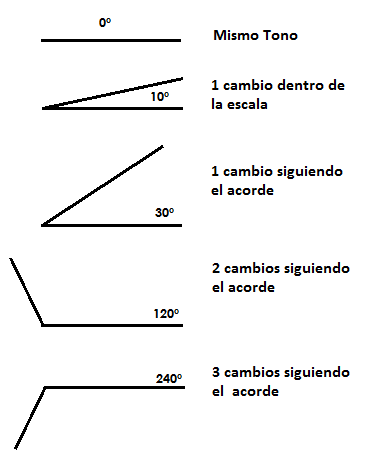
\includegraphics[scale=0.75]{graphics/tabla-corresp-Tono-Angulo.png}
		\caption{Tabla correspondencias entre ángulos y cambios de tono}
		\label{fig:Figura3Voz1}
		\end{figure}

De este modo si la diferencia de ángulos es menor a 10º se sigue usando el mismo tono, si la diferencia está entre 10º y 30º se usa el tono adyacente dentro de la escala. Si está entre 30º y 120º el primer tono más cercano del acorde, entre 120º y 240º el segundo tono más cercano del acorde y hasta 360º el tercer tono más cercano del acorde. El acorde que se usa es el acorde fundamental del tono que da el color de la figura. Esta relación se basa en la asociación que tiene Scriabin con los colores \cite{ScriabinQuintasColor}: él hace corresponder un color a un tono y a su acorde fundamental sin distinguir entre acorde mayor o menor para cada una de las notas de la escala cromática.

	\item Sintetizar las notas: Mismo procedimiento que en la anterior versión.

\end{itemize}

Un ejemplo completo de composición sobre una figura de entrada (Figura~\ref{fig:Figura0Voz1}) usando la segunda versión del algoritmo (ComposerFigMelody2): \\

		\begin{figure}[!htbp]
		\centering
		\hspace*{0.0in}
		
\includegraphics[scale=1.0]{graphics/simpletest1.png}
		\caption{Figura de entrada}
		\label{fig:Figura0Voz1}
		\end{figure}

\begin{itemize}

	\item Procesar la figura (Figura~\ref{fig:Figura1Voz1}): Ordenamos los vértices (identificados con números) y hallamos la longitud de los lados. \\

		\begin{figure}[!htbp]
		\centering
		\hspace*{0.0in}
		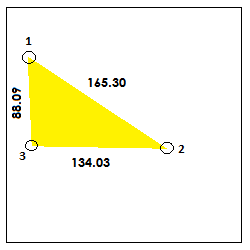
\includegraphics[scale=1.0]{graphics/simpletest1-F1.png}
		\caption{Figura de entrada con los vértices ordenados y con las longitudes de los lados}
		\label{fig:Figura1Voz1}
		\end{figure}

	\item Calcular duraciones (Figura~\ref{fig:Figura2Voz1}): Se puede apreciar cómo el lado más largo obtiene una duración mayor (blanca) que los otros dos lados (negra). A pesar de que los dos lados más pequeños tienen diferentes longitudes, se ha aproximado su valor a una misma duración.\\
		
		\begin{figure}[!htbp]
		\centering
		\hspace*{0.0in}
		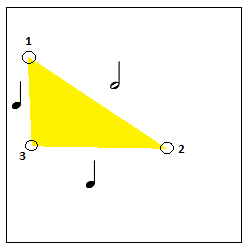
\includegraphics[scale=1.0]{graphics/simpletest1-F2.png}
		\caption{Figura de entrada con el ritmo producido}
		\label{fig:Figura2Voz1}
		\end{figure}

	\item Obtener tonos  (Figura~\ref{fig:Figura4Voz1}): Para conseguirlo primero se tiene que ver qué nota corresponde al color de la figura (en este caso se usa la correspondencia propuesta por Scriabin en la que el amarillo es D ``re''). Una vez se tiene la nota y su ángulo, se calcula la diferencia entre el nuevo ángulo y el anterior, el resultado es negativo por lo que se tiene que bajar de tono y como la diferencia en valor absoluto está entre los 10º y 30º, sólo se baja un escalón en la escala actual (en este ejemplo escala de Re Mayor), obteniendo la nueva nota: C ``do''. \\
Para conseguir el tercero y último tono, se calcula la diferencia del último vértice restando el ángulo del tercer vértice con el del segundo. Se obtiene un valor positivo luego se tiene que subir el tono. Al estar entre 30º y 120º se sube de un salto en el acorde de nota fundamental el color de la figura (en este caso es el acorde de D ``re'': D - F ``fa''- A ``la''). Como no se está en el acorde con el último tono obtenido (C ``do'') se viaja al tono más cercano que pertenezca al acorde, es decir, D ``re''. Y de ahí como la diferencia de ángulos es positiva se va a hacer un salto ascendente (a tono superior) de una unidad dentro del acorde, se pasa al tono F ``fa''.
	
		\begin{figure}[!htbp]
		\centering
		\hspace*{0.0in}
		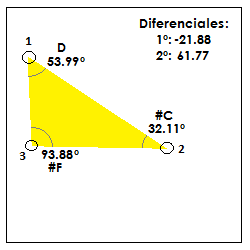
\includegraphics[scale=1.0]{graphics/simpletest1-F3.png}
		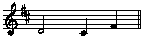
\includegraphics[scale=1.0]{graphics/simpletest1-MELpartitura.png}
		\caption{Figura de entrada con los ángulos y los tonos que produce}
		\label{fig:Figura4Voz1}
		\end{figure}

	\item Sintetizar las notas (Partitura de Figura~\ref{fig:Figura4Voz1}): Se tienen las duraciones y se tienen los tonos. Sólo falta juntarlos para crear las notas teniendo en cuenta el orden de los vértices.\\

\end{itemize}

Y con la misma figura (Figura~\ref{fig:Figura0Voz1}), vemos cual sería la salida de la primera versión del algoritmo (ComposerFigMelody1):

\begin{itemize}
	
	\item Procesar la figura (Figura~\ref{fig:Figura1Voz1}): Este proceso es el mismo en ambas versiones. \\
	
	\item Calcular duraciones (Figura~\ref{fig:Figura5Voz1}): Se puede ver cómo el algoritmo es más fiel a la correspondencia de las longitudes de los lados con las duraciones. Ahora los lados que antes tenían la misma duración, son distintos con una pequeña diferencia.\\
		
		\begin{figure}[!htbp]
		\centering
		\hspace*{0.0in}
		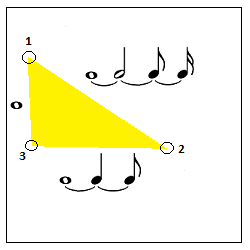
\includegraphics[scale=1]{graphics/simpletest1-F2_2.png}
		\caption{Figura de entrada con los lados y el ritmo conseguido}
		\label{fig:Figura5Voz1}
		\end{figure}

	\item Obtener tonos  (Figura~\ref{fig:Figura6Voz1}): En esta versión el algoritmo es de correspondencia directa entre el ángulo del vértice y el tono. Al igual que en el anterior algoritmo, el primer tono lo determina el color de la figura. Después se tiene el ángulo del segundo vértice que es pequeño y por tanto genera un pequeño salto en el tono. El tercer vértice tiene un ángulo mucho mayor y como se puede observar, se da un salto mayor respecto al anterior tono.
	
		\begin{figure}[!htbp]
		\centering
		\hspace*{0.0in}
		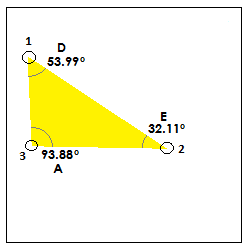
\includegraphics[scale=1]{graphics/simpletest1-F3_2.png}
		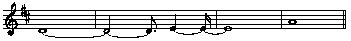
\includegraphics[scale=1]{graphics/simpletest1_2-MELpartitura.png}
		\caption{Figura de entrada con los ángulos y los tonos producidos}
		\label{fig:Figura6Voz1}
		\end{figure}

	\item Sintetizar las notas (Partitura de Figura~\ref{fig:Figura6Voz1}): El mismo proceso que en el algoritmo de la segunda versión.

\end{itemize}

%----------------------------------------------------------------------------------------------------------------------------------------------------

\subsection{2ª Voz: Melodía Secundaria}

La segunda voz sirve de acompañamiento a la primera. Se usa la misma estructura que a la hora de componer la melodía principal aunque con algunos cambios. Además se necesita el segmento de melodía principal como entrada para poder basarse en ella a la hora de componer, pudiendo conseguir resultados que siguen las bases armónicas de la música.

\begin{itemize}
	\item Procesar la figura: Esta fase será la misma que la usada en la primera voz.

	\item Calcular duraciones: Se usa el mismo proceso que la segunda versión de la primera voz pero en este caso se añade un paso más. Las duraciones obtenidas se adaptan para que el total sea la longitud pedida y nunca mayor que el segmento de la melodía. Además, si la duración total del acompañamiento es menor que la de la voz principal, hay que decidir en qué momento de la melodía va a empezar el acompañamiento.

	\item Obtener tonos: Respecto al anterior algoritmo, en este apartado se sigue sacando una correlación entre los ángulos y los tonos, pero se añade un proceso intermedio. Mientras se generan los tonos se analiza el comportamiento de la segunda voz respecto a la melodía principal y si es necesario, se aplican pequeñas variaciones para disminuir las disonancias que puedan aparecer al juntar ambas voces. Estos cambios, que siguen los principios de las técnicas más básicas del contrapunto, se activan cuando el intervalo entre la primera y la segunda voz es disonante y además se mantiene un periodo alargado en el tiempo. \\
Las variaciones aplicadas intentarán que los cambios sean mínimos, por ejemplo, si un tono ha bajado pero lo ha hecho a un tono disonante de larga duración respecto a la primera voz entonces se cambia el tono por otro que esté lo más cerca del original.

	\item Sintetizar las notas: Se sigue el mismo algoritmo pero con un añadido. Hay que tener en cuenta que la segunda voz puede tener una duración menor que la primera voz. Para que sea consistente la composición, todas las voces tienen que tener la misma duración y por tanto hay que rellenar con silencios la parte que falta a la segunda voz.

\end{itemize}

Veamos un ejemplo con la siguiente figura de entrada (Figura~\ref{fig:Figura0Voz2}):

		\begin{figure}[!htbp]
		\centering
		\hspace*{0.0in}
		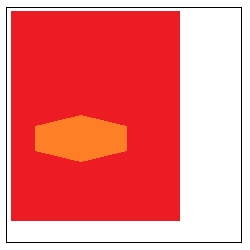
\includegraphics[scale=1]{graphics/simpletest4.png}
		\caption{Figuras de entrada para componer con la figura interior}
		\label{fig:Figura0Voz2}
		\end{figure}

\begin{itemize}

	\item Procesar la figura: Igual que en los anteriores ejemplos se calcula la longitud de los lados de la figura y el orden de los vértices.

	\item Calcular duraciones (Figuras ~\ref{fig:Figura1Voz2} y ~\ref{fig:Figura2Voz2}): En la primera figura vemos las duraciones obtenidas sin adaptar y en la segunda figura se puede observar cómo la duración de algunos lados ha disminuido para conseguir la duración deseada.

 		\begin{figure}[!htbp]
		\centering
		\hspace*{0.0in}
		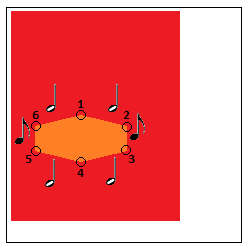
\includegraphics[scale=1]{graphics/simpletest4-F2.png}
		\caption{Figuras de entrada con los lados de la figura interior y las duraciones obtenidas sin adaptación}
		\label{fig:Figura1Voz2}
		\end{figure}

		\begin{figure}[!htbp]
		\centering
		\hspace*{0.0in}
		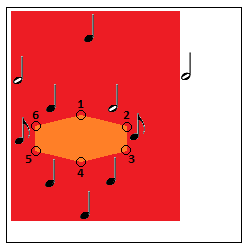
\includegraphics[scale=1]{graphics/simpletest4-F2_2.png}
		\caption{Figuras de entrada con la duración de la figura exterior y con las duraciones adaptadas de la interior}
		\label{fig:Figura2Voz2}
		\end{figure}

	\item Obtener tonos (Figuras ~\ref{fig:Figura3Voz2} y ~\ref{fig:Figura4Voz2}): En la primera figura podemos observar los tonos generados sin usar técnicas de contrapunto. La tercera y sexta nota generada produce una disonancia de larga duración (negra) con la voz principal. Si se aplican las técnicas contrapuntísticas \color{red}(Poner en glosario? o en Apendice? o aqui mismo decir algo?) \color{blue}podemos comprobar cómo se han cambiado por un tono cercano sin perder la idea del salto de tono que nos indicaba el ángulo de los vértices.

		\begin{figure}[!htbp]
		\centering
		\hspace*{0.0in}
		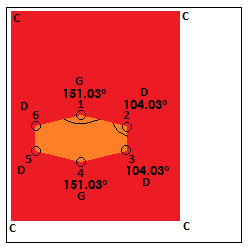
\includegraphics[scale=1]{graphics/simpletest4-F3.png}
		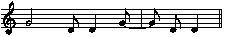
\includegraphics[scale=1]{graphics/simpletest4-F3-MEL2partitura.png}
		\caption{Figuras de entrada con los ángulos y los tonos producidos sin técnicas contrapuntísticas}
		\label{fig:Figura3Voz2}
		\end{figure}

		\begin{figure}[!htbp]
		\centering
		\hspace*{0.0in}
		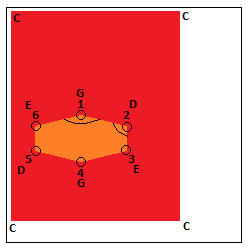
\includegraphics[scale=1]{graphics/simpletest4-F3_2.png}
		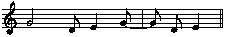
\includegraphics[scale=1]{graphics/simpletest4-F3_2-MEL2partitura.png}
		\caption{Figuras de entrada con los ángulos y los tonos producidos con técnicas contrapuntísticas}
		\label{fig:Figura4Voz2}
		\end{figure}

	\item Sintetizar las notas (Partitura de Figura~\ref{fig:Figura4Voz2}): Igual que la primera voz pero añadimos silencios si son necesarios. En este ejemplo no son necesarios.

\end{itemize}

%----------------------------------------------------------------------------------------------------------------------------------------------------

\subsection{3ª Voz: Bajo}

El bajo es la voz que se encarga de mantener la armonía de la pieza musical compuesta. Por tanto se ha optado por una estructura sencilla. \\

El algoritmo desarrollado consiste en usar siempre notas de una misma duración (por defecto redondas) cuyo tono sea el color de la figura de entrada y cuya duración sea la de la figura dada (Figura~\ref{fig:Figura1Voz3}). Si las duraciones no son suficientes para rellenar la duración total, se termina usando una duración menor para la última nota. \\

		\begin{figure}[!htbp]
		\centering
		\hspace*{0.0in}
		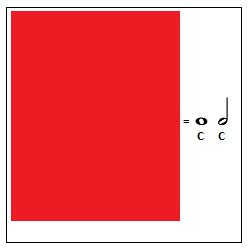
\includegraphics[scale=1]{graphics/simpletest2-F2F3.png}
		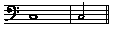
\includegraphics[scale=1]{graphics/simpletest2-BASSpartitura.png}
		\caption{Figura de entrada con los tonos producidos}
		\label{fig:Figura1Voz3}
		\end{figure}

Otra posibilidad habilitada para el bajo es usar el algoritmo de la primera voz de forma experimental, pero transportando los tonos una o varias octavas más grave (Figura~\ref{fig:Figura2Voz3}). El número de octavas depende del tono más agudo y del tono más grave de la melodía compuesta evitando que al transportar la melodía se salga del límite de representación de las notas.

		\begin{figure}[!htbp]
		\centering
		\hspace*{0.0in}
		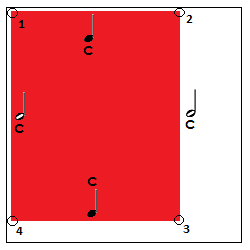
\includegraphics[scale=1]{graphics/simpletest2-F2F3_2.png}
		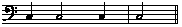
\includegraphics[scale=1]{graphics/simpletest3_2-BASSpartitura.png}
		\caption{Figura de entrada con los tonos producidos}
		\label{fig:Figura2Voz3}
		\end{figure}

%----------------------------------------------------------------------------------------------------------------------------------------------------

\subsection{4ª Voz: Ritmo}

La cuarta voz será la encargada de la parte de percusión dentro de la pieza musical.

El algoritmo desarrollado se inspira en el concepto de inestabilidad de una figura de A. Pintado \cite{portutesis}. Separamos el proceso en 3 pasos:

\begin{itemize}
	\item Asignación de vértices: Primero se crea un ritmo que consiste en pulsos largos de duración configurable (por defecto redondas). A cada pulso le es asignado una serie de vértices dependiendo de la densidad de vértices de la figura (a mayor número de vértices, se le asignarán más a cada pulso). Hay que tener en cuenta que los vértices están ordenados como en los anteriores algoritmos.

	\item Calcular círculo equivalente: Se calcula el círculo de área equivalente a la figura dada. Este círculo tendrá el mismo área y de centro el punto de equilibrio de la figura de entrada (Figura~\ref{fig:Figura2Voz4}).
		
		\begin{figure}[!htbp]
		\centering
		\hspace*{0.0in}
		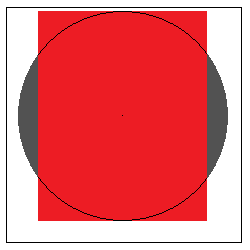
\includegraphics[scale=1]{graphics/simpletest2-Circulo.png}
		\caption{Figura de entrada y el círculo equivalente}
		\label{fig:Figura2Voz4}
		\end{figure}

	\item Dividir el ritmo: Después se va calculando cuanta desviación tienen los vértices respecto al perímetro del círculo. A mayor distancia, mayor desviación y por tanto mayor inestabilidad (Figura~\ref{fig:Figura3Voz4}). La inestabilidad produce que el ritmo se subdivida en más notas de menor duración (Figura~\ref{fig:Figura4Voz4}).

		\begin{figure}[!htbp]
		\centering
		\hspace*{0.0in}
		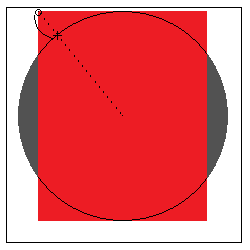
\includegraphics[scale=1]{graphics/simpletest2-Circulo_2.png}
		\caption{Figura de entrada con el círculo equivalente y la desviación del primer vértice}
		\label{fig:Figura3Voz4}
		\end{figure}

		\begin{figure}[htbp]
		\centering
		\hspace*{0.0in}
		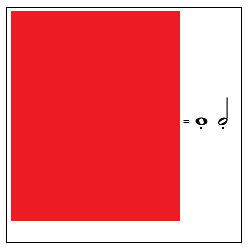
\includegraphics[scale=1]{graphics/simpletest2-F2F3_3.png}
		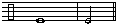
\includegraphics[scale=1]{graphics/simpletest2-PERpartitura.png}
		\caption{Figura de entrada y los ritmos producidos}
		\label{fig:Figura4Voz4}
		\end{figure}

\end{itemize}

%----------------------------------------------------------------------------------------------------------------------------------------------------

\subsection{Mezclador de voces}

Los anteriores algoritmos sirven para crear un trozo de música de una voz a partir de una figura, el siguiente paso es juntar las distintas voces para formar una pieza musical completa, para ello se utiliza el ``Mezclador''. 
Este algoritmo se puede dividir en tres pasos diferentes. Actualmente se tienen dos diferentes versiones:

La primera versión del Mezclador sólo tiene en cuenta la primera voz (melodía) y la cuarta (ritmo).

\begin{itemize}
	\item Ordenar las figuras: Lo primero que se hace es ordenar las figuras según su relevancia. Para conseguirlo se utiliza un parámetro de vistosidad que se calcula a partir de tres características importantes de cada figura:
	\begin{itemize}
		\item La primera es lo llamativo que es el color de la figura. Se descompone el color en sus tres componentes principales RGB y se da peso a cada una de ellas. Luego este valor se multiplica por la saturación del color.
		\item La segunda componente es el área que ocupa la figura. Cuanto más grande sea, más vistosa es.
		\item La tercera componente es la distancia que tiene del centro de la imagen. El ojo humano enfoca de centro a laterales cuando ve una imagen por primera vez, por ello tiene más vistosidad una figura que se encuentra en el centro de la imagen que en un lateral o esquina.
	\end{itemize}
	
\color{blue}
	La fórmula con los pesos de cada componente es la siguiente:
	\begin{center}
		$vistosidad(Figura) =
		A*rgb.saturation * (rgb.red*pR + rgb.green*pG + rgb.blue*pB)
		 + B*area + C*distanceCenter
		$
	\end{center}

donde pR = 0.45, pG = 0.35 y pB = 0.20 son las constantes de influencia de cada color básico obtenidas de forma experimental. Y las constantes A = 0.5, B = 0.3 y C = 0.2 son los valores de importancia de cada atributo de la figura.
\color{black}

	\item Componer voces: Tras haber ordenado las figuras por vistosidad se va componiendo con cada una de forma iterativa las distintas voces. En este caso solo se compone la melodía y el ritmo con cada una de las figuras.

	\item Mezclar voces: Una vez tenemos todas las voces compuestas las juntamos y creamos la pieza musical añadiendo todos los parámetros necesarios (tempo, armadura de clave, título de la pieza musical, ...).

\end{itemize}

En la segunda versión del Mezclador, se tienen en cuenta las cuatro voces disponibles. Por ello tendrá más complejidad que la primera versión.

\begin{itemize}
	\item Ordenar las figuras: Este primer paso se hace de la misma forma que la primera versión.

	\item Componer voces: Para la segunda versión del Mezclador se van a diferenciar dos tipos de figuras: figuras padre y figuras hija. Las llamadas figuras hija son aquellas que se localizan dentro de otra figura. Las figuras hija pueden tener a su vez otras figuras hija. Las figuras padre son aquellas que no forman parte de otra figura (es decir, no son hijas de ninguna figura) y pueden contener figuras hija. Es fácil de clasificarlas por la estructura arbórea en la que están organizadas.

Una vez las tenemos clasificadas vamos iterando por cada figura padre componiendo su melodía, bajo y ritmo y si tiene alguna figura hija, entonces también se añade la segunda melodía dando como entrada al algoritmo de composición de acompañamiento (segunda voz) la figura hija y la melodía ya compuesta. Por cada figura interior (hija) se compone un nuevo bloque de la figura padre con diferentes acompañamientos.

	\item Mezclar voces: Se realiza de la misma forma que la primera versión del Mezclador.

\end{itemize}

Veamos un ejemplo de la segunda versión del algoritmo, para simplificar se usará las figuras vistas anteriormente (Figura~\ref{fig:Figura0Mixer}).

		\begin{figure}[!htbp]
		\centering
		\hspace*{0.0in}
		
\includegraphics[scale=1]{graphics/simpletest5.png}
		\caption{Figuras de entrada}
		\label{fig:Figura0Mixer}
		\end{figure}

\begin{itemize}
	\item Ordenar las figuras: Se ordenan las figuras de tal forma que en primer lugar está el rectángulo rojo, en segundo lugar el triángulo amarillo y al final el hexágono irregular.

	\item Componer voces (Figura~\ref{fig:Figura1Mixer}): Primero se compone la voz principal, bajo y ritmo de la figura padre, que en este caso es el rectángulo. Después para cada figura hija (triángulo y hexágono) se compone su acompañamiento. Se puede observar en la partitura cómo primero se introduce el trozo correspondiente al rectángulo con el triángulo y que seguidamente se compone el trozo del rectángulo con el hexágono.

		\begin{figure}[!htbp]
		\centering
		\hspace*{0.0in}
		
\includegraphics[scale=1]{graphics/simpletest5.png}
		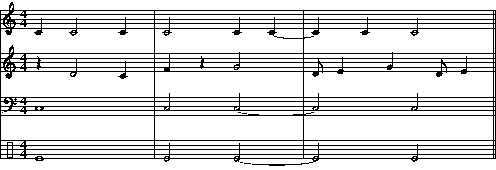
\includegraphics[scale=0.8]{graphics/simpletest5-partitura.png}
		\caption{Figuras de entrada con las voces producidas}
		\label{fig:Figura1Mixer}
		\end{figure}

	\item Mezclar voces (Partitura de Figura~\ref{fig:Figura1Mixer}): Por último se añaden las voces correctamente a la pieza musical y se rellenan los valores de los atributos necesarios para crear la partitura y el archivo de audio midi.

\end{itemize}
